\documentclass{beamer} 

\usepackage[utf8]{inputenc}
\usepackage[T1]{fontenc}
\usepackage{graphicx}
\usepackage{multicol}

\usetheme{Berlin}
\begin{document}

\title{Git - sistem za kontrolu verzija}
\author{Stefan Nožinić (stefan@lugons.org)}

\frame{
\titlepage
}

\frame{
	\frametitle{Uvod}
	\begin{itemize} 
		\item Šta je sistem za kontrolu verzija?
		\item Problemi prilikom razvoja softvera
		\itemize{
			\item Ko je napravio promenu?
			\item kad?
		}
		\item Repozitorijum - mesto za skladištenje koda
	\end{itemize}
}

\frame{
	\frametitle{Vrste sistema za kontrolu verzija}
	\begin{itemize} 
		\item Centralizovani - SVN 
		\item Distribuirani - Git
	\end{itemize}
}

\frame{
	\frametitle{Git}
	\begin{itemize}
		\item open source 
		\item Razvijen od strane Linus Torvaldsa - kreatora Linuksa 
	\end{itemize}
}

\frame{
	\frametitle{Stanja u Git-u}
	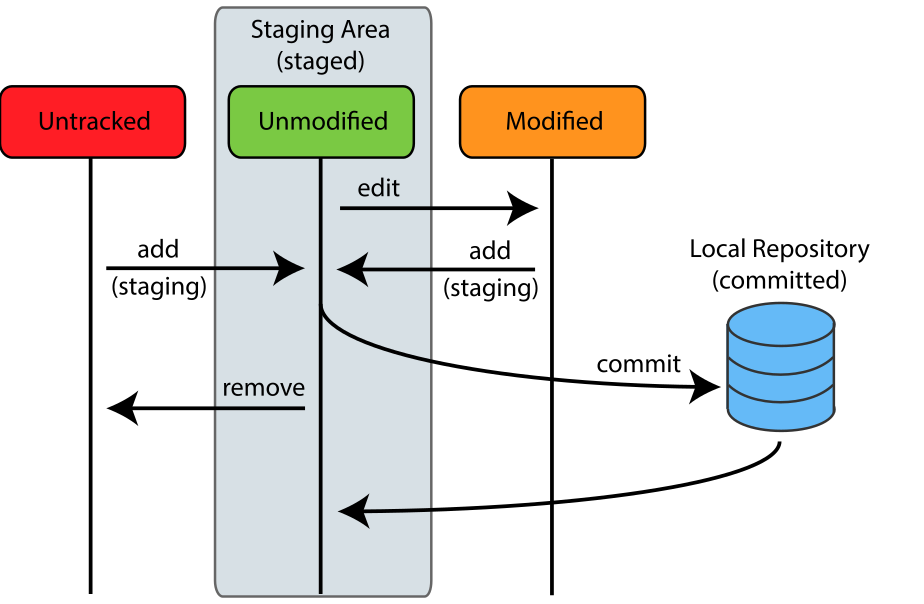
\includegraphics{git.png}
}

\frame{
	\frametitle{Osnovne operacije u repozitorijumu}
	\begin{itemize}
		\item Inicijalizacija repozitorijuma 
		\item Dodavanja fajlova u repozitorijum 
		\item git commit 
		\item git commit --amend - dodavanje na postojeći komit
		\item Pregled izmena, log i diff 
		\item git reset --hard 
		\item git reset --hard HEAD~1 - brisanje komita
	\end{itemize}
}

\frame{
	\frametitle{Grananje}
	\begin{itemize}
		\item Upotrebljava se kada je potrebno razvijati novu stavku u softveru 
		\item Može da služi kao i metod da se više stavki razvija paralelno bez toga da zavise jedna od druge 
		\item korisno za testiranje različitih metoda za istu namenu 
		\item Korisno za uklanjanje grešaka
	\end{itemize}
}


\frame{
	\frametitle{Rad sa granama}
	\begin{itemize}
		\item git checkout -b nova-grana
		\item git checkout postojeca-grana
		\item git branch -d nova-grana 
		\item git merge grana 
	\end{itemize}
}

\frame{
	\frametitle{Dobre prakse}
	\begin{itemize}
		\item Imati dev granu za netestiranu verziju dok master ostaviti za stabilnu verziju
		\item Svaka nova komponenta u softveru se razvija u posebnoj feature grani za tu komponentu
		\item Kada se razvoje komponente završi, radi se merge u dev granu 
		\item Kada je nova verzija spremna, pravi se release-x.y grana 
		\item dev -> release-x.y
		\item Ako se pronađe bug dok je razvoj spreman za objavu (release grana), pravi se hotfix grana i u njoj se ispravljaju greške 
		\item hotfix -> release-x.y 
		\item release-x.y -> dev, dev -> master 
		\item Dodati tag sa git tag x.y da se označi nova verzija 
	\end{itemize}
}

\frame{
	\frametitle{Kloniranje, ažuriranje i slanje izmena na server}
	\begin{itemize}
		\item git clone - kloniranje postojećeg repozitorijuma sa servera
		\item git pull - update lokalnog repozitorijuma
		\item git push - slanje izmena na repozitorijum
		\item git push <remote> <branch> - slanje izmena na zadati server na zadatu granu na datom serveru
		\item git remote -v - listanje svih povezanih servera
		\item git remote add <name> <adresa> - dodavanja remote servera
		\item Servisi za deljenje koda: GitHub, GitLab, BitBucket, ...
	\end{itemize}
}

\end{document}
